\documentclass[a4paper, 12pt, titlepage]{article}

\usepackage{natbib}
\usepackage[utf8]{inputenc}
\usepackage{graphics}
\usepackage{graphicx}     
\usepackage[french]{babel}
\usepackage{eurosym}
\usepackage[pdftex,colorlinks=true,linkcolor=blue,citecolor=blue,urlcolor=blue]{hyperref}
\usepackage{geometry}
\usepackage{icomma}
% \usepackage{cite} % cite et natbib redéfinissent tous les deux \cite
\usepackage{float}
\usepackage[nottoc, notlof, notlot]{tocbibind}
\usepackage[OT1]{fontenc}
\usepackage{hyperref}
\usepackage{xurl}
\usepackage{csquotes}
\usepackage{caption}
\usepackage{subcaption}
\usepackage{titling}
\usepackage{titlepic}
\usepackage[utf8]{inputenc}

\newcommand{\Note}[1]{\textit{\textbf{Note :} #1}}
\newcommand{\CO}[0]{\texorpdfstring{CO$_2$}{CO2} }

\geometry{top=2cm, bottom=2cm, left=2cm, right=2cm}
\setlength{\parskip}{0.5em} % Espace entre les paragraphes, 1em = largeur moyenne d'1 caractère
\setcounter{page}{-1}

\begin{titlepage}
    
\title{
    AP4B : Rapport de conception
    \break\break
    
\includegraphics[width=5cm, height=5cm]{images/logo.png}
}
\author{
    Clovis BURGAUD
    \and Julien CONSTANT 
    \and Noé ÉCHARD  
    \and Cyrille STROESSER
}

\date{7 Janvier 2022}

\end{titlepage}

\pagestyle{plain}

\begin{document}
    
\maketitle

\section*{Introduction}
\addcontentsline{toc}{section}{Introduction}

Pour ce projet d’AP4B en Java nous avons décidé de choisir le sujet "Sim Power" et ainsi
de recréer un classique des jeux de gestion avec notamment la gestion d’énergie au centre du gameplay de ce dernier.
Dans ce rapport, nous allons vous présenter les règles de base et les fonctionnalités de notre jeu, ensuite vous pourrez voir les différents diagrammes UML qui servent à décrire plus en détail le fonctionnement du jeu et du code. Enfin Nous vous présenterons le fonctionnement du groupe durant la réalisation de ce projet et les outils utilisés afin de s’organiser efficacement.

Notre code source est disponible ici : \url{https://github.com/CyrilleStr/AP4B}


\newpage
\tableofcontents

\newpage
\section{Règle du jeu}

Le but du jeu est de garder le bonheur (« happiness ») des habitants au-dessus de 0 le plus longtemps possible. Pour cela , les habitations doivent être suffisamment alimentées en énergie et non polluées. Le joueur perd quand le bonheur arrive à zéro, son score équivaut au nombre de jours qu’ils a pu tenir.

Tous les bâtiments doivent obligatoirement être accessibles et donc placés à côté d’une route, les nouvelles routes placées doivent également suivre des routes déjà existantes.

\textbf{Production d’Energie :} 
	Il existe 2 types de bâtiments produisant de l’énergie : les « fossil plants » (centrale à gaz, charbon) et les renouvelables (solaire, éolien, hydraulique). Les « fossil plants » nécessitent d’être alimentés en ressources qui sont dispersées autour de la carte et peuvent être extraites grâce à des mines. L’activité de ces « fossil plants » induit de la pollution sur les 9 cases autour de celle-ci.
	
\textbf{Consommation d’énergie :}
	Deux types de bâtiments consomment également de l’énergie : les mines et les maisons. Une fois l’énergie de la journée produite, elle est d’abord distribuée aux mines en fonction de leurs besoin et l’énergie qui reste est ensuite divisée entre les maisons. Le bonheur est basé sur l’énergie que ces maisons reçoivent.
	
\textbf{Gestion de l’argent :}
	Au début du jeu, le joueur commence avec une somme d’argent qui lui permet de commencer à placer des bâtiments. Pour continuer à en gagner, il doit garder les habitants heureux car le bonheur est rapport de l’argent gagné par les maisons chaque jour. En plus du coût de placement des bâtiments, les centrales et les mines ont un « servicing cost » ou coût d’entretien qui consomme de l’argent chaque jour.
	
\textbf{Bâtiments inactifs :}
	Un bâtiment peut devenir inactif de 2 manières soit il n’a plus assez d’énergie pour fonctionner, soit son coût d’entretien est supérieur à l’argent disponible. Une fois inactif il ne produit plus de ressources ni d’énergie.
	
\textbf{Gestion du bonheur :}
	Le bonheur des habitant est basé sur le niveau d’alimentation en énergie des maisons. Exemple : Si la quantité d’énergie requise est atteinte à 100\% le bonheur de la maison est à 100\%, si elle n’est atteinte qu’à 30\%, la maison aura un niveau de bonheur de 30\%. Le bonheur global est la moyenne du bonheur de toutes les maisons. Si une maison est dans un nuage de pollution d’une « fossil plant », son bonheur baisse automatiquement de 5 points.


\newpage
\section{Diagrammes use-cases}

Le diagramme de Use case du menu principal se présente de la manière suivante :
\begin{figure}[H]
    \centering
    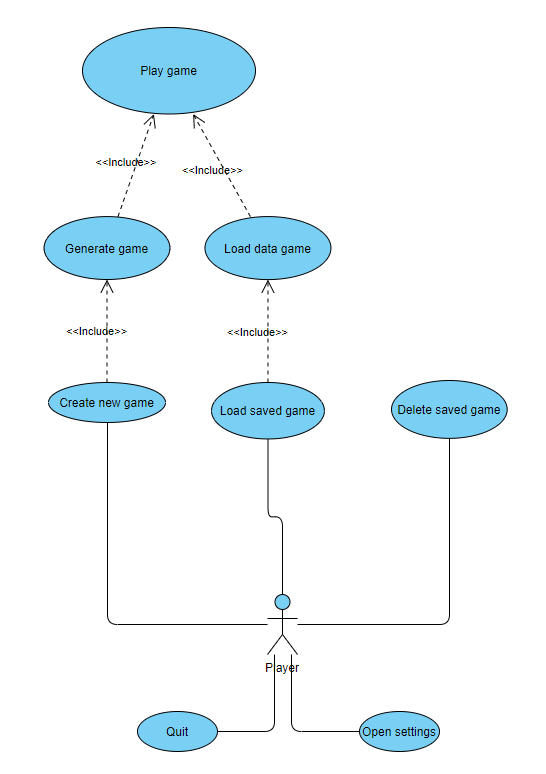
\includegraphics[width=0.5\linewidth]{images/useCaseMenu.png}
    \caption{Diagramme de use case du menu principal}
    \label{fig:useCaseMenu}
\end{figure}
Le joueur se trouve face à 5 possibilités représentées par 5 boutons : quitter le jeu, aller dans les paramètres, supprimer une partie sauvegardée, charger une partie sauvegardée ou créer une nouvelle partie.
\pagebreak

Le diagramme de use case du jeu se présente de la manière suivante :
\begin{figure}[H]
    \centering
    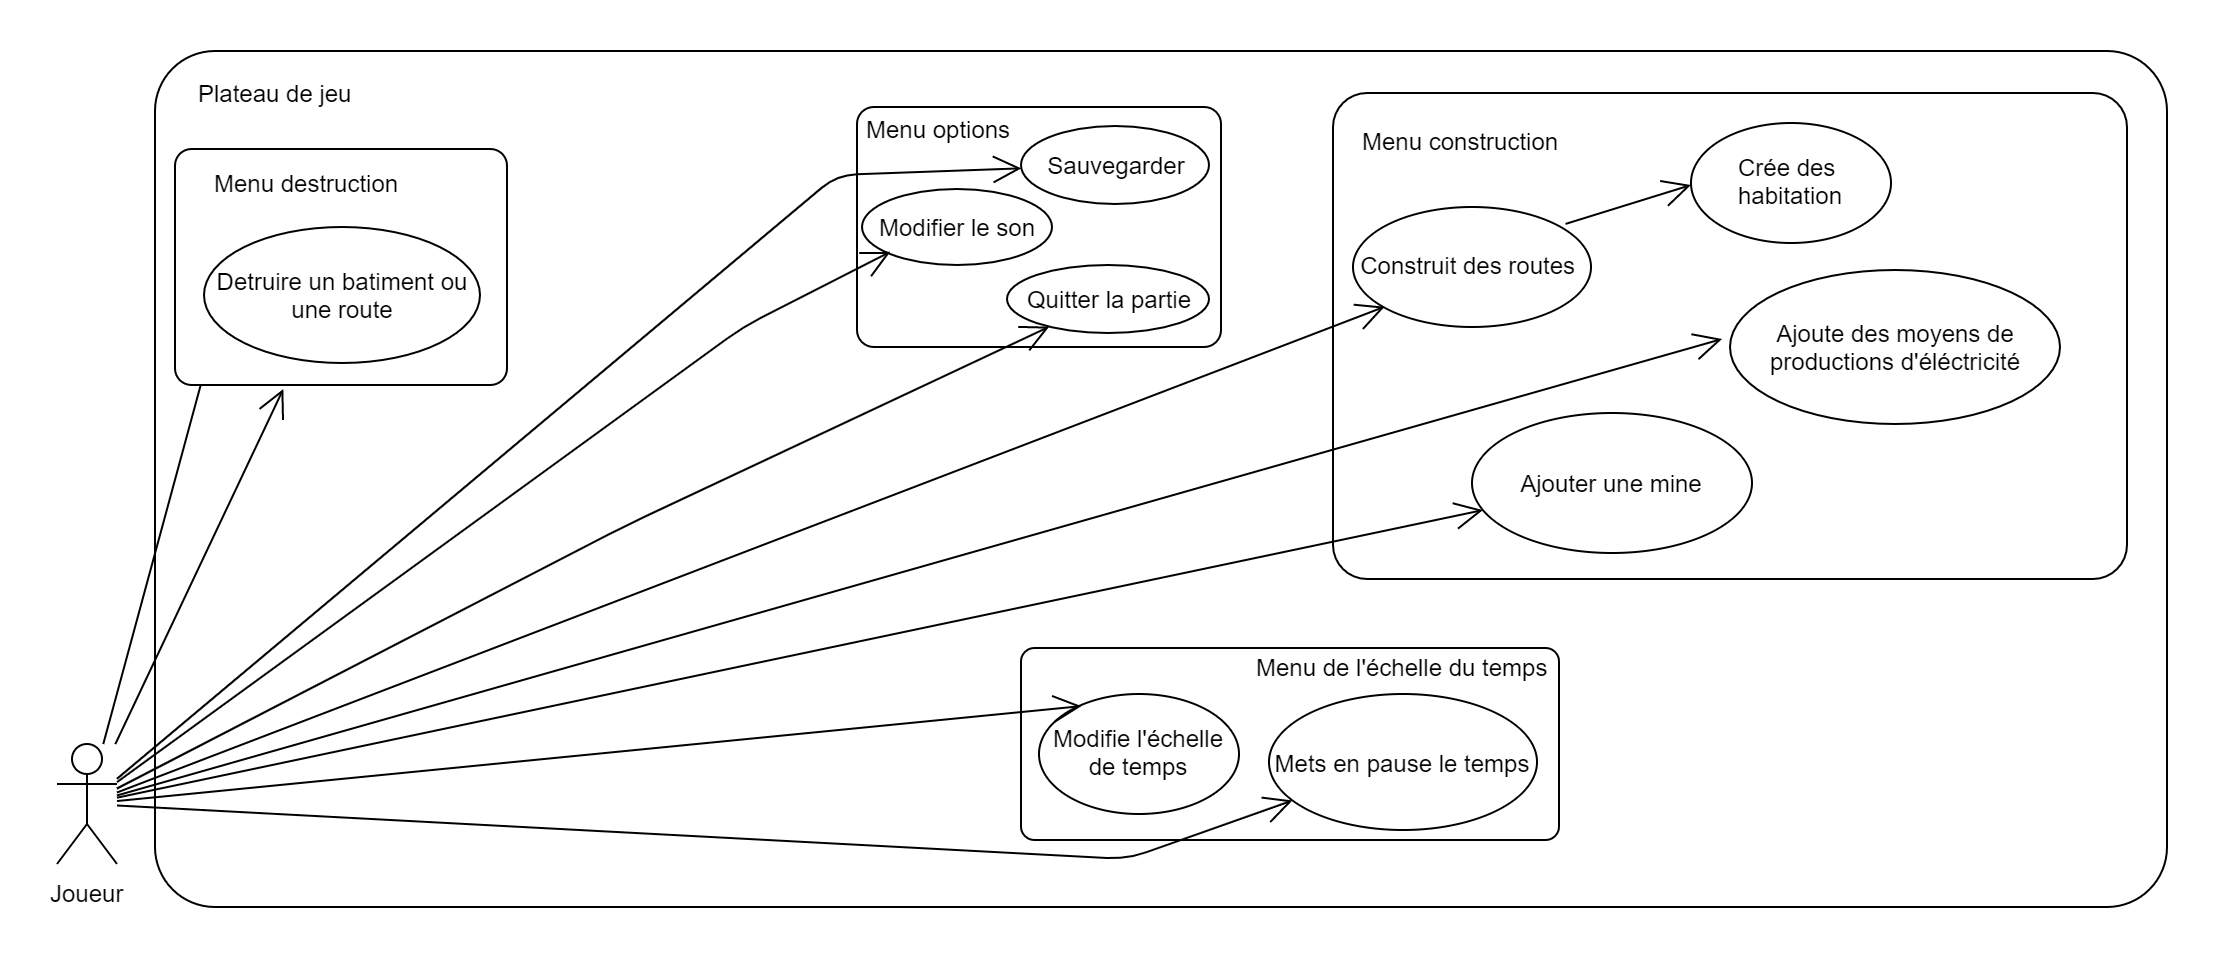
\includegraphics[width=1\linewidth]{images/Use-cases-1.png}
    \caption{Diagramme de use case en jeu}
    \label{fig:useCaseEnJeu}
\end{figure}
Afin de gérer sa ville le joueur et sa partie, le joueur peut faire 4 catégories d'actions séparées dans 4 menus.
Il peut soit :
\begin{itemize}
    \item[\textbullet] accélérer, ralentir ou mettre en pause le temps en jeu
    \item[\textbullet] détruire ce qu'il a construit
    \item[\textbullet]changer les paramètres du jeu si il ne l'a pas fait dans le menu principal
    \item[\textbullet]construire bâtiments, maisons et routes pour développer sa ville
\end{itemize}

\newpage
\section{Diagramme de classe}

\begin{figure}[H]
    \centering
    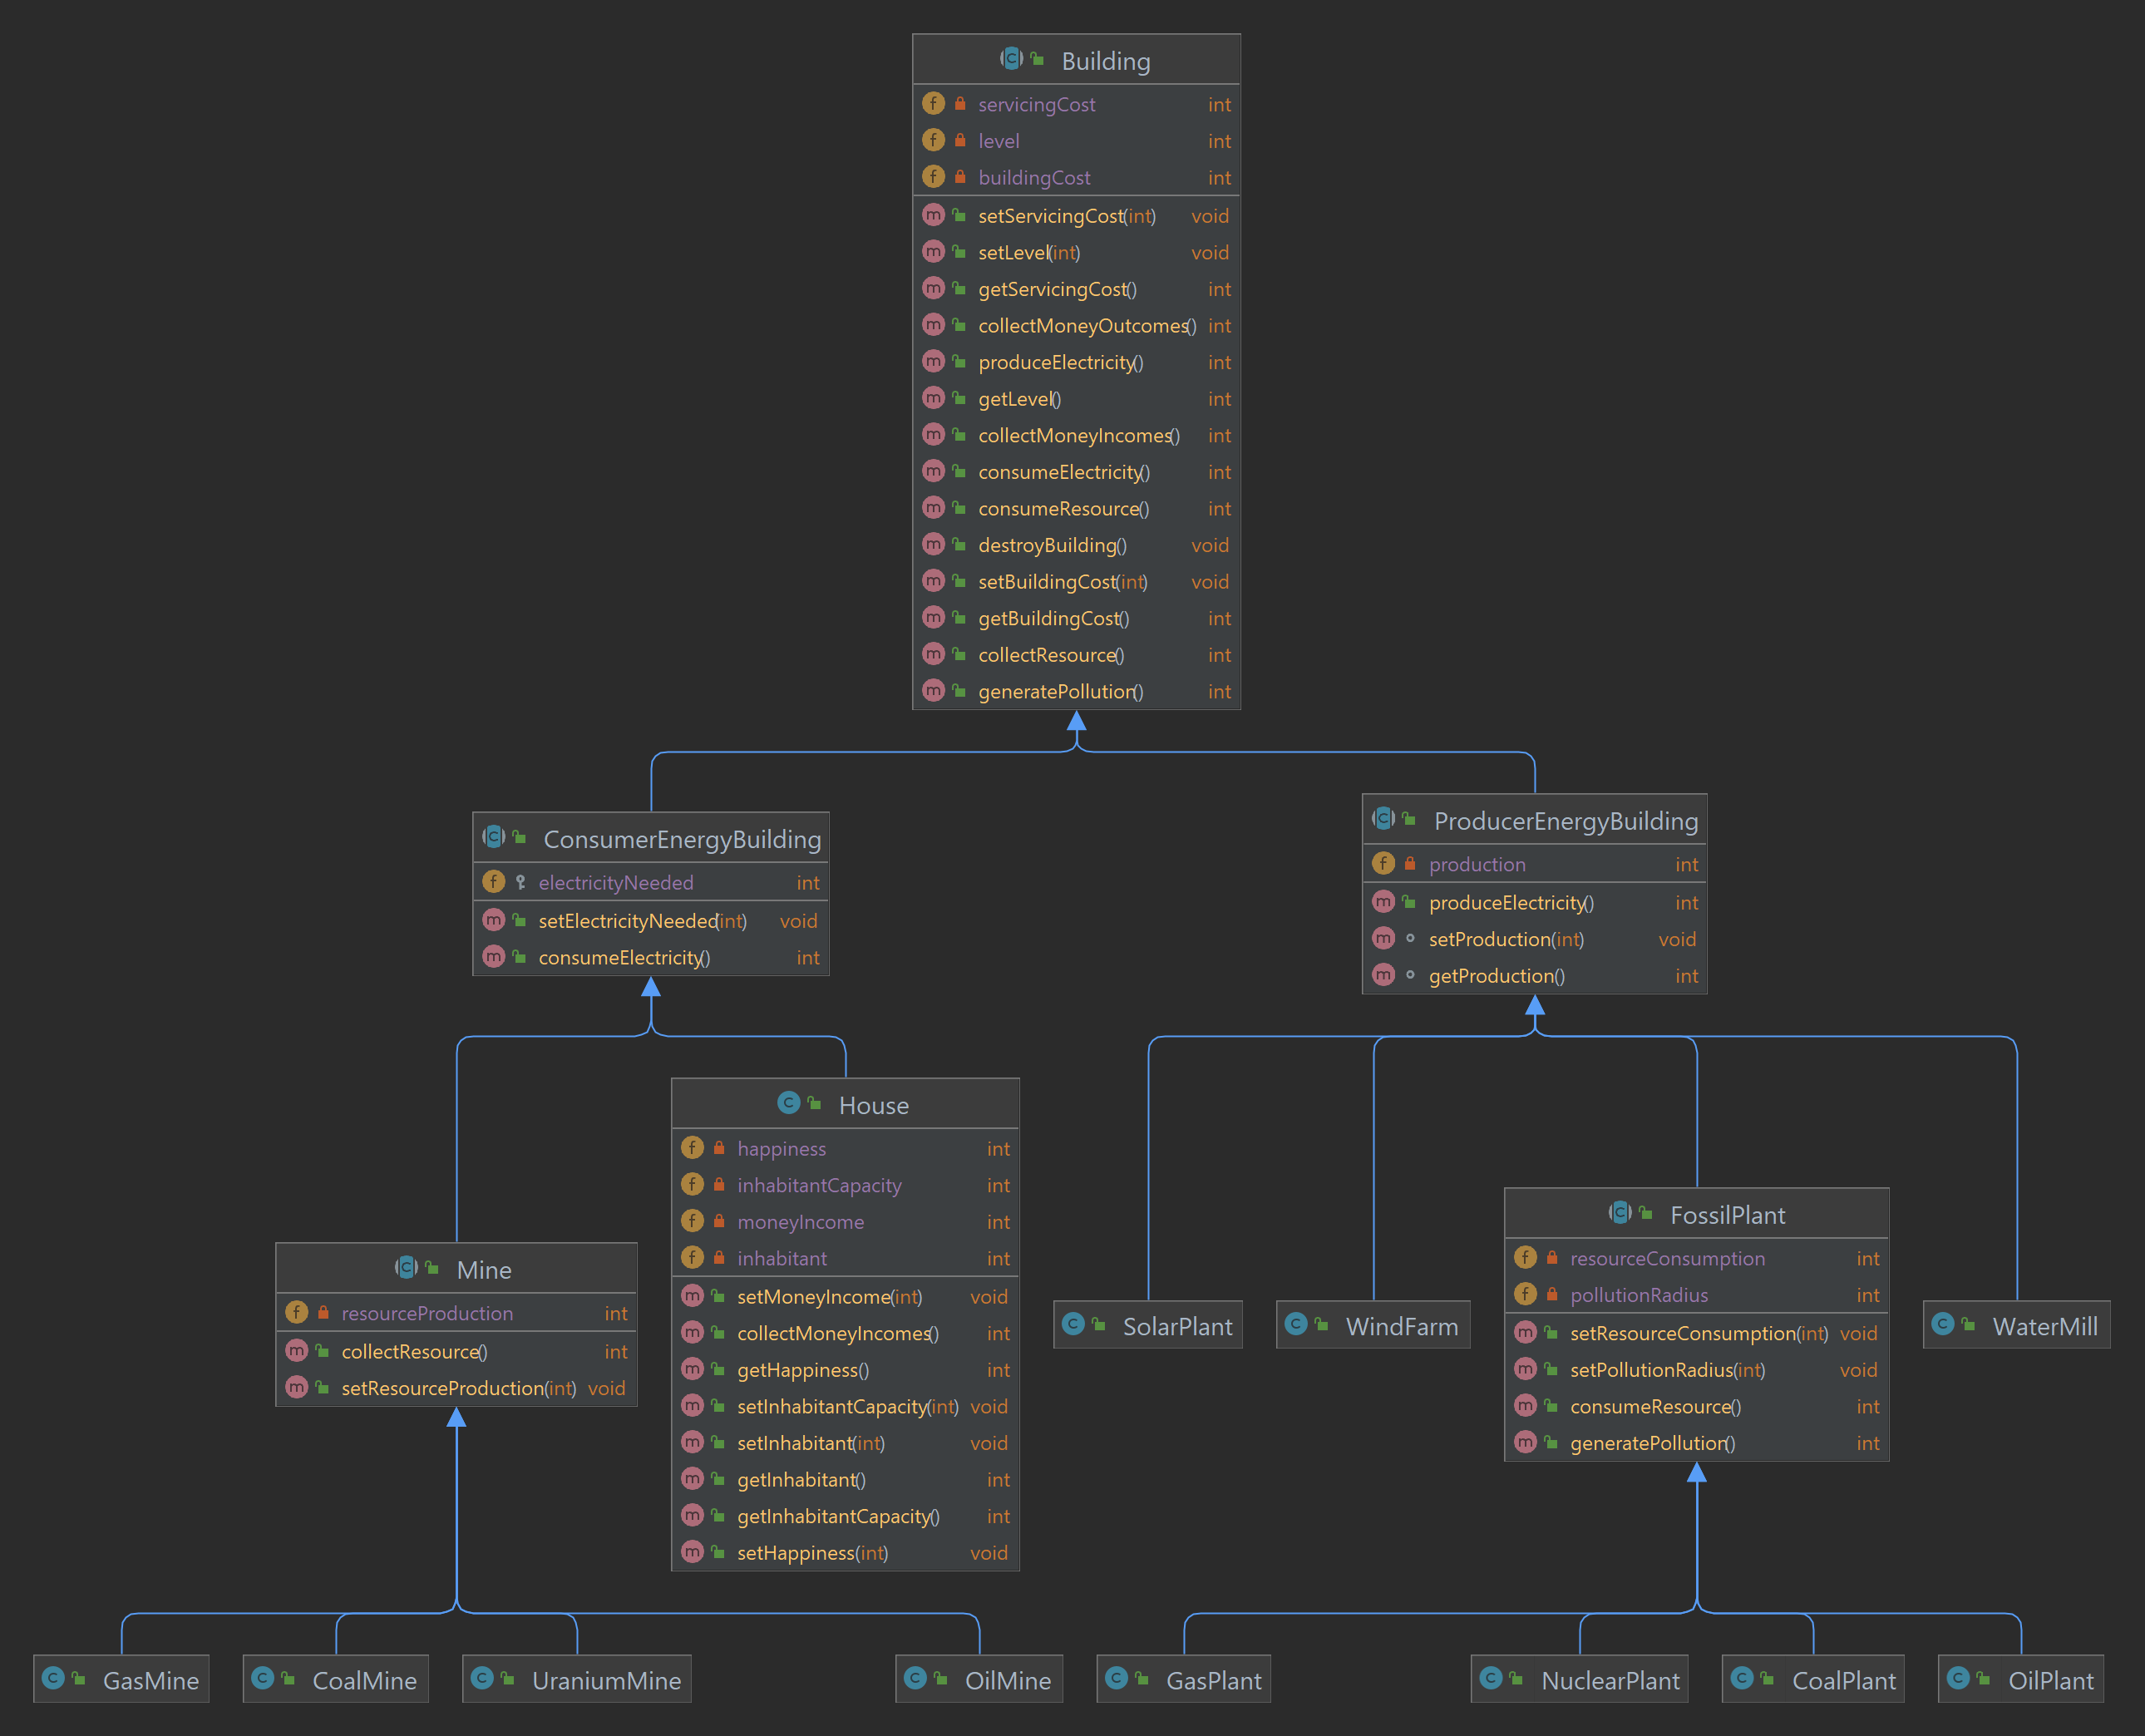
\includegraphics[width=1\linewidth]{images/classBuidling.png}
    \caption{Diagramme de classe de la partie bâtiment}
    \label{fig:classBuilding}
\end{figure}

\begin{figure}[H]
    \centering
    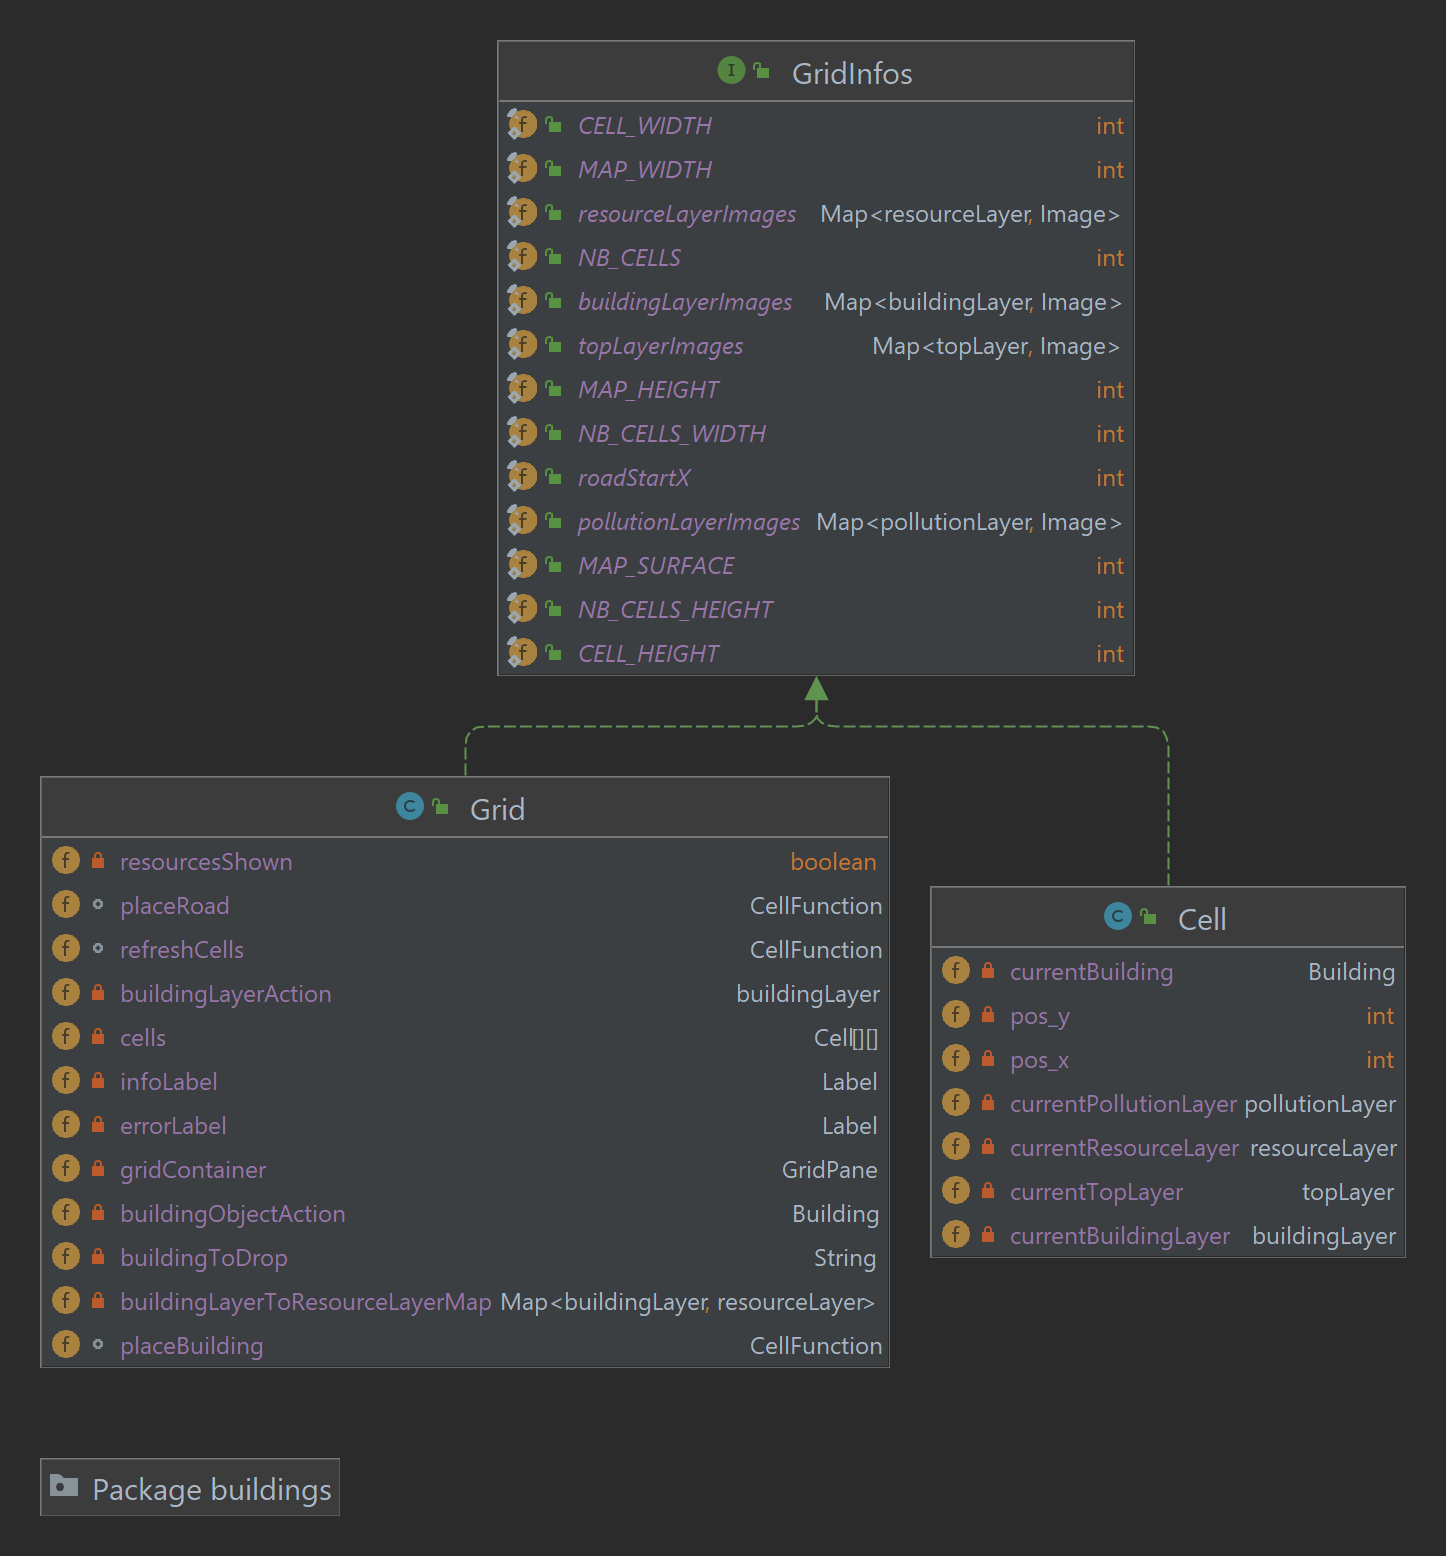
\includegraphics[width=1\linewidth]{images/classGrid.png}
    \caption{Diagramme de classe de la partie gestion de la carte}
    \label{fig:classGrid}
\end{figure}

\begin{figure}[H] %C'est la que faut changer l'image
    \centering
    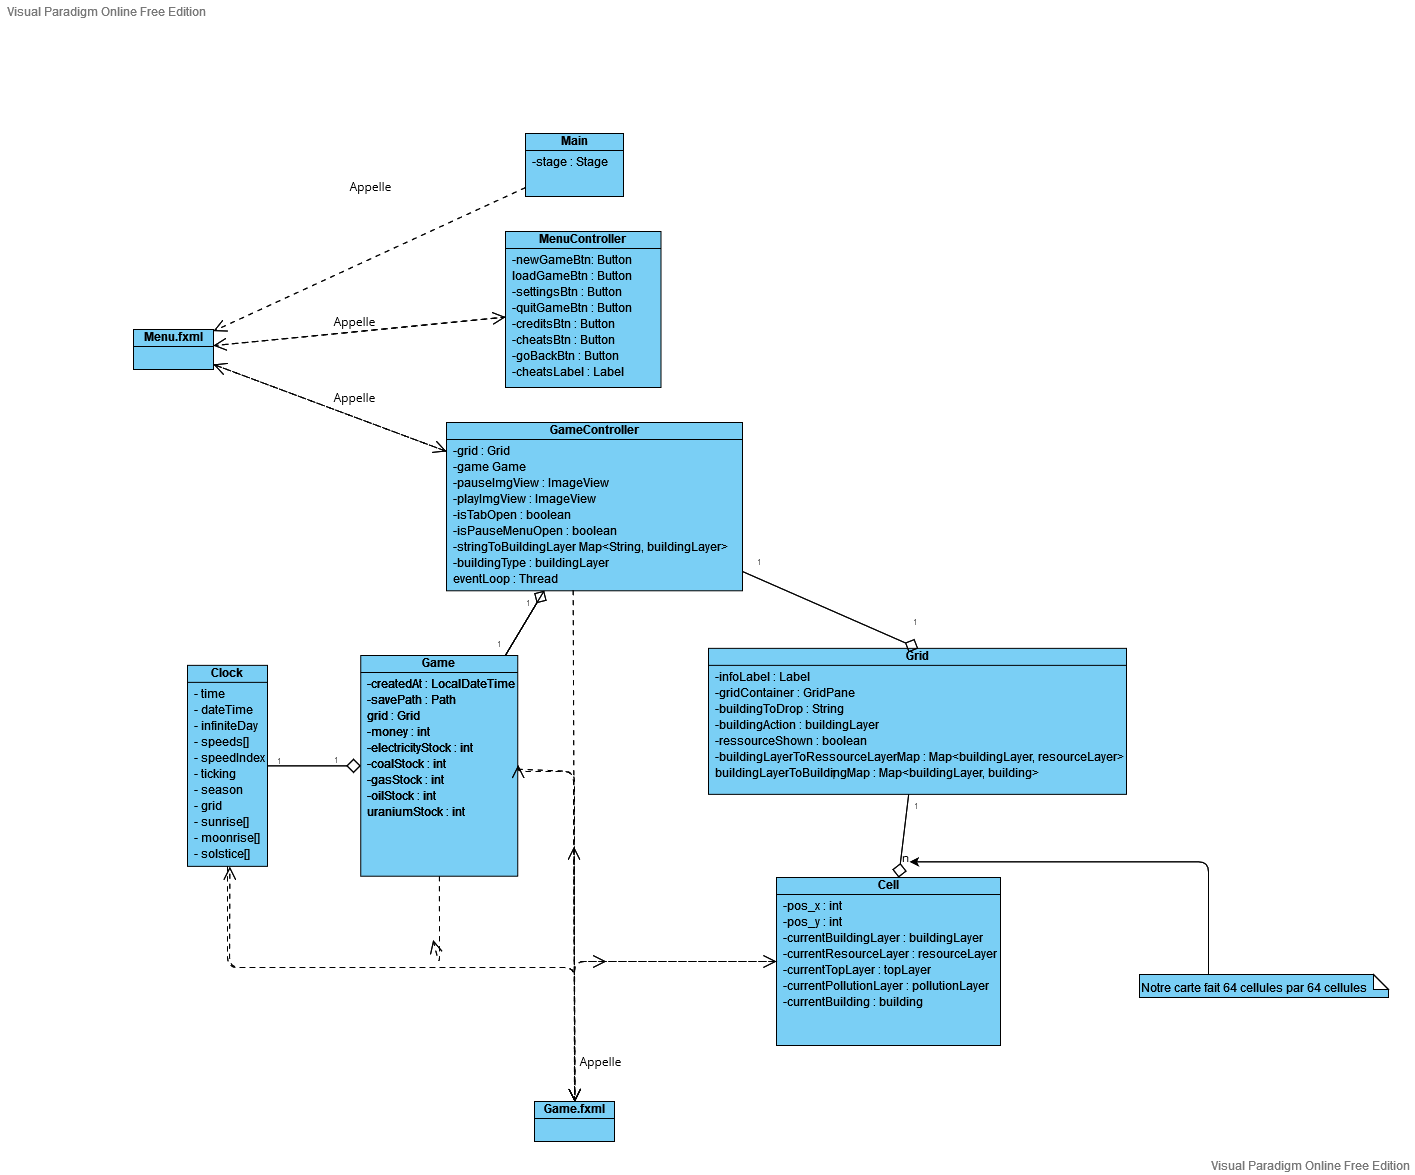
\includegraphics[width=1\linewidth]{images/classGlobal.png}
    \caption{Diagramme de classe global du jeu}
    \label{fig:classGlobal}
\end{figure}

\newpage
\section{Diagrammes de séquence}

Le diagramme de séquence "boucle d'évenements", présente le fonctionnement du moteur de jeu. Appelé par le \textit{gameController}, l'\textit{eventLoop} va vérifier que temps s'écoule bien, et si c'est le cas, cette boucle va appeler la classe \textit{game} à exécuter un certain nombre de méthodes. Si le temps ne s'écoule pas il ne se passe absolument rien. La classe \textit{game} va parcourir chaque bâtiment et appeler certaines méthodes en fonction du type de bâtiments. Par exemple, si le bâtiment est une mine, les méthodes \textit{collectResource()}, \textit{collectMoneyOutcomes()} et \textit{consumeElectricity()}. La classe \textit{game} va alors récupérer les valeurs retournées et actualiser respectivement les ressources, l'argent et l'électricité.

\begin{figure}[H]
    \centering
    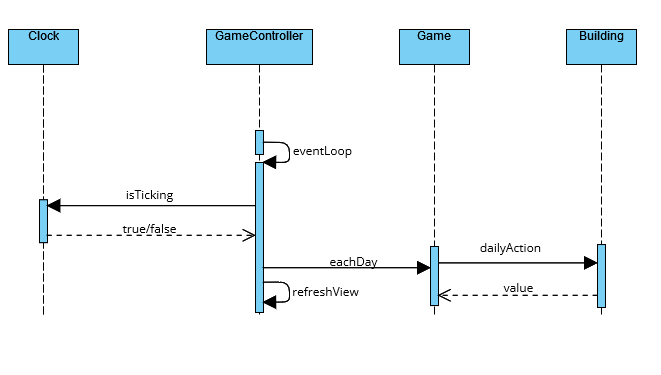
\includegraphics[width=1\linewidth]{images/eventLoop.png}
    \caption{Diagramme de séquence de la boucle d'évènement}
    \label{fig:sequenceEvent}
\end{figure}

\pagebreak

Le digramme "pose de bâtiment", présente l'enchaînement de méthodes appelées lorsqu'un joueur essaye de poser un bâtiment.

\begin{figure}[H]
    \centering
    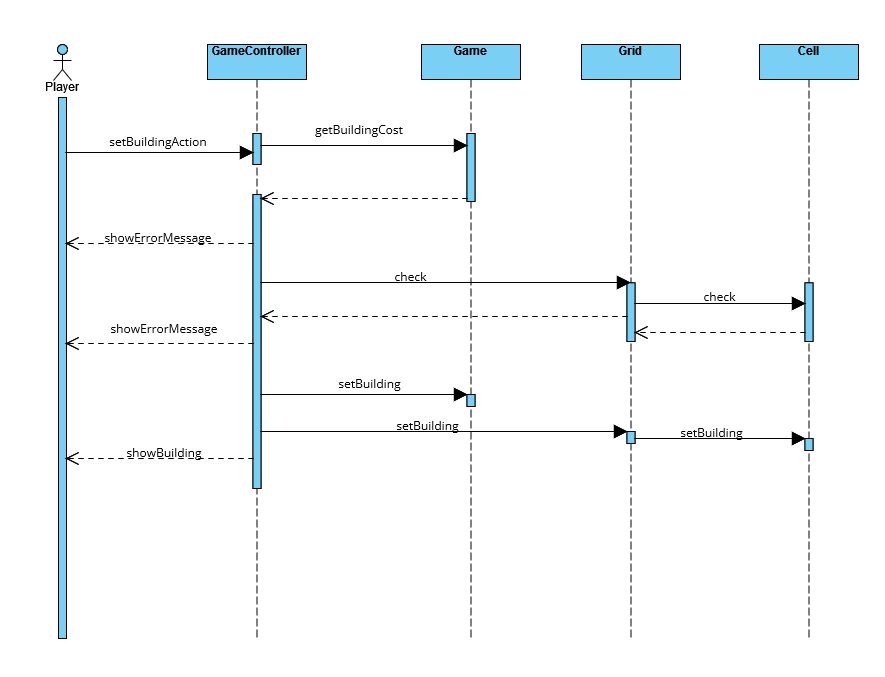
\includegraphics[width=1\linewidth]{images/setBuilding.png}
    \caption{Diagramme de séquence de la pose de bâtiment}
    \label{fig:sequenceBuilding}
\end{figure}


\newpage
\section{Fonctionnement du groupe}

Notre groupe étant composé de quatre personnes, ils nous a paru crucial d'avoir une organisation bien claire et bien structuré en tout point. Nous nous sommes inspiré du fonctionnement des entreprises pour s'organiser. Voici quelque explications.

\begin{itemize}
    \item[\textbullet]
    \textbf{Outils utilisés} : 
    Nous avons créé un serveur Discord pour communiquer facilement et structurer nos échanges lors d'appel ou de messages. Nous avons choisi l'IDE \textit{Intellij}, dans la mesure où il est disponible gratuitement pour les étudiants et facile d'utilisation, il comprend beaucoup de fonctionnalités intéressantes tel que CodeWithMe, permettant de programmer à plusieurs en temps réel, la génération automatique des diagrammes à partir des classes Java et inversement pour une meilleure vue d'ensemble du projet et un bon gestionnaire de Git. Pour la bibliothèque graphique, nous avons opté pour \textit{JavaFX} car cette bibliothèque est nativement supportée par Intellij et permet l'édition des scènes très simplement via le logicel \textit{SceneBuilder} développé pour cela. Il permet de générer des vues en fichier \enquote{.fxml} qui sont ensuite utilisés par JavaFX pour afficher du contenu.
    \linebreak
    
    \item[\textbullet]
    \textbf{Protocoles} : 
    Pour éviter au maximum les conflits et pour garder en permanence une version exploitable de notre programme nous avons décidé d'attribuer une branche de développement \textit{git} par personne et de ne jamais ajouter du code directement sur la branche \textit{main}. À chaque nouvelle ajout de fonctionnalité, nous devions le faire sur notre branche respective et faire une \textit{pull request} pour signaler cet ajout. Puis au moins un autre membre devait vérifier les changements et valider cette \textit{pull request}. Ainsi, le programme de la branche \textit{main} possède une version stable et fonctionnelle.
    \linebreak
    
    \item[\textbullet]
    \textbf{Planification} :
    Dès le commencement de l'UV \textit{AP4B} nous avons planifié des réunions hebdomadaires le mardi matin. Ces réunions nous permettaient de prendre des décisions sur la conception, de poser des questions lors des Travaux Pratiques et de se répartir des tâches jusqu'à la prochaine réunion. Évidemment à l'approche de la date limite du rendu, des réunions supplémentaires se sont imposées afin de convenir et de respecter les délais.
    \linebreak
    
    \item[\textbullet]
    \textbf{Étapes} : nous avons réaliser ce projet en plusieurs étapes. Tous d'abord il a fallu transcrire toutes nos idées par écrit et faire un tris en fonction de la faisabilité de chacune. Puis, il a fallut dessiner nos diagrammes en commençant par les Use-Case. Après avoir rédiger un premier diagramme des classes nous avons commencé à coder. La priorité était d'implémenter la génération d'une carte et le temps. Puis nous avons ajouté des bâtiments et la gestions des ressources. Tout au long de la réalisation nous avons constamment remis en question le diagramme des classes et les use-cases. Ayant atteint nos objectifs avant les vacances de Noël, nous avons prévu d'implémenter des fonctionnalités \enquote{bonus}, mais utiles, pendant les vacances.
\end{itemize}
    
\newpage
\newpage
\newpage
\section{Conclusion}

Ce projet a été pour nous un très bon moyen d'améliorer nos compétences en Programmation Orientée Objet. Grâce à celui-ci, nous avons pu améliorer notre capacité à travailler en groupe, à distribuer le travail, à nous organiser mais également montrer ce que l'on pouvait faire.

Nous sommes contents de ce que nous avons pu accomplir jusqu'à maintenant, que ce soit du point de vue de la conception ou du point de vue du développement. Nous considérons ce projet comme un succès dans la mesure où nous pensons que le temps qui nous a été accordé va nous permettre de finir notre jeu à temps tout en respectant les objectifs demandés.

Pour finir, nous voulons remercier Mohammed Kas et Franck Gechter pour nous avoir permis de connaître les bases de la Programmation Orientée Objet en Java à travers l'UV d'AP4B.
\newpage

\nocite{*}
\bibliography{bibliographie}{}
\bibliographystyle{plain}

\listoffigures

\end{document}
